\documentclass[a4paper, 11pt]{article}

\usepackage{subfiles}

\usepackage[utf8]{inputenc}

\usepackage[
backend=biber,
style=alphabetic,
sorting=ynt
]{biblatex}
 
\addbibresource{bibliography.bib}

\usepackage{textcomp}
\usepackage[T1]{fontenc}
\usepackage{multirow}
\usepackage{float}
\usepackage[caption = false]{subfig}
\usepackage{longtable}
\usepackage{listings}
\usepackage{mathtools}
\DeclareMathOperator{\tr}{Tr}
\usepackage{commath}
\usepackage{bbold}
\usepackage{xcolor}
\usepackage{physics}
%\usepackage[margin=1.8cm]{geometry}

\usepackage{tikz-cd} 
\usepackage{amsmath}
\usepackage{amsfonts}
\usepackage{amssymb}
\usepackage{amsthm}
\usepackage{graphicx}
\usepackage[colorinlistoftodos]{todonotes}
\usepackage[colorlinks=true, allcolors=blue]{hyperref}
\usepackage{siunitx}
\sisetup{separate-uncertainty=true}

\usepackage[sc]{mathpazo}
\linespread{1.05}         % Palladio needs more leading (space between lines)
\usepackage[T1]{fontenc}

\newcommand{\diag}[1]{\text{diag}\qty(#1)}
\newcommand{\Lagr}{\mathcal{L}}
\newcommand{\const}{\text{const}}
\newcommand{\sign}[1]{\text{sign}\qty(#1)}

\title{On the radiation emitted by radially symmetric BH accretion}
\author{Jacopo Tissino}
\date{2019}

\begin{document}

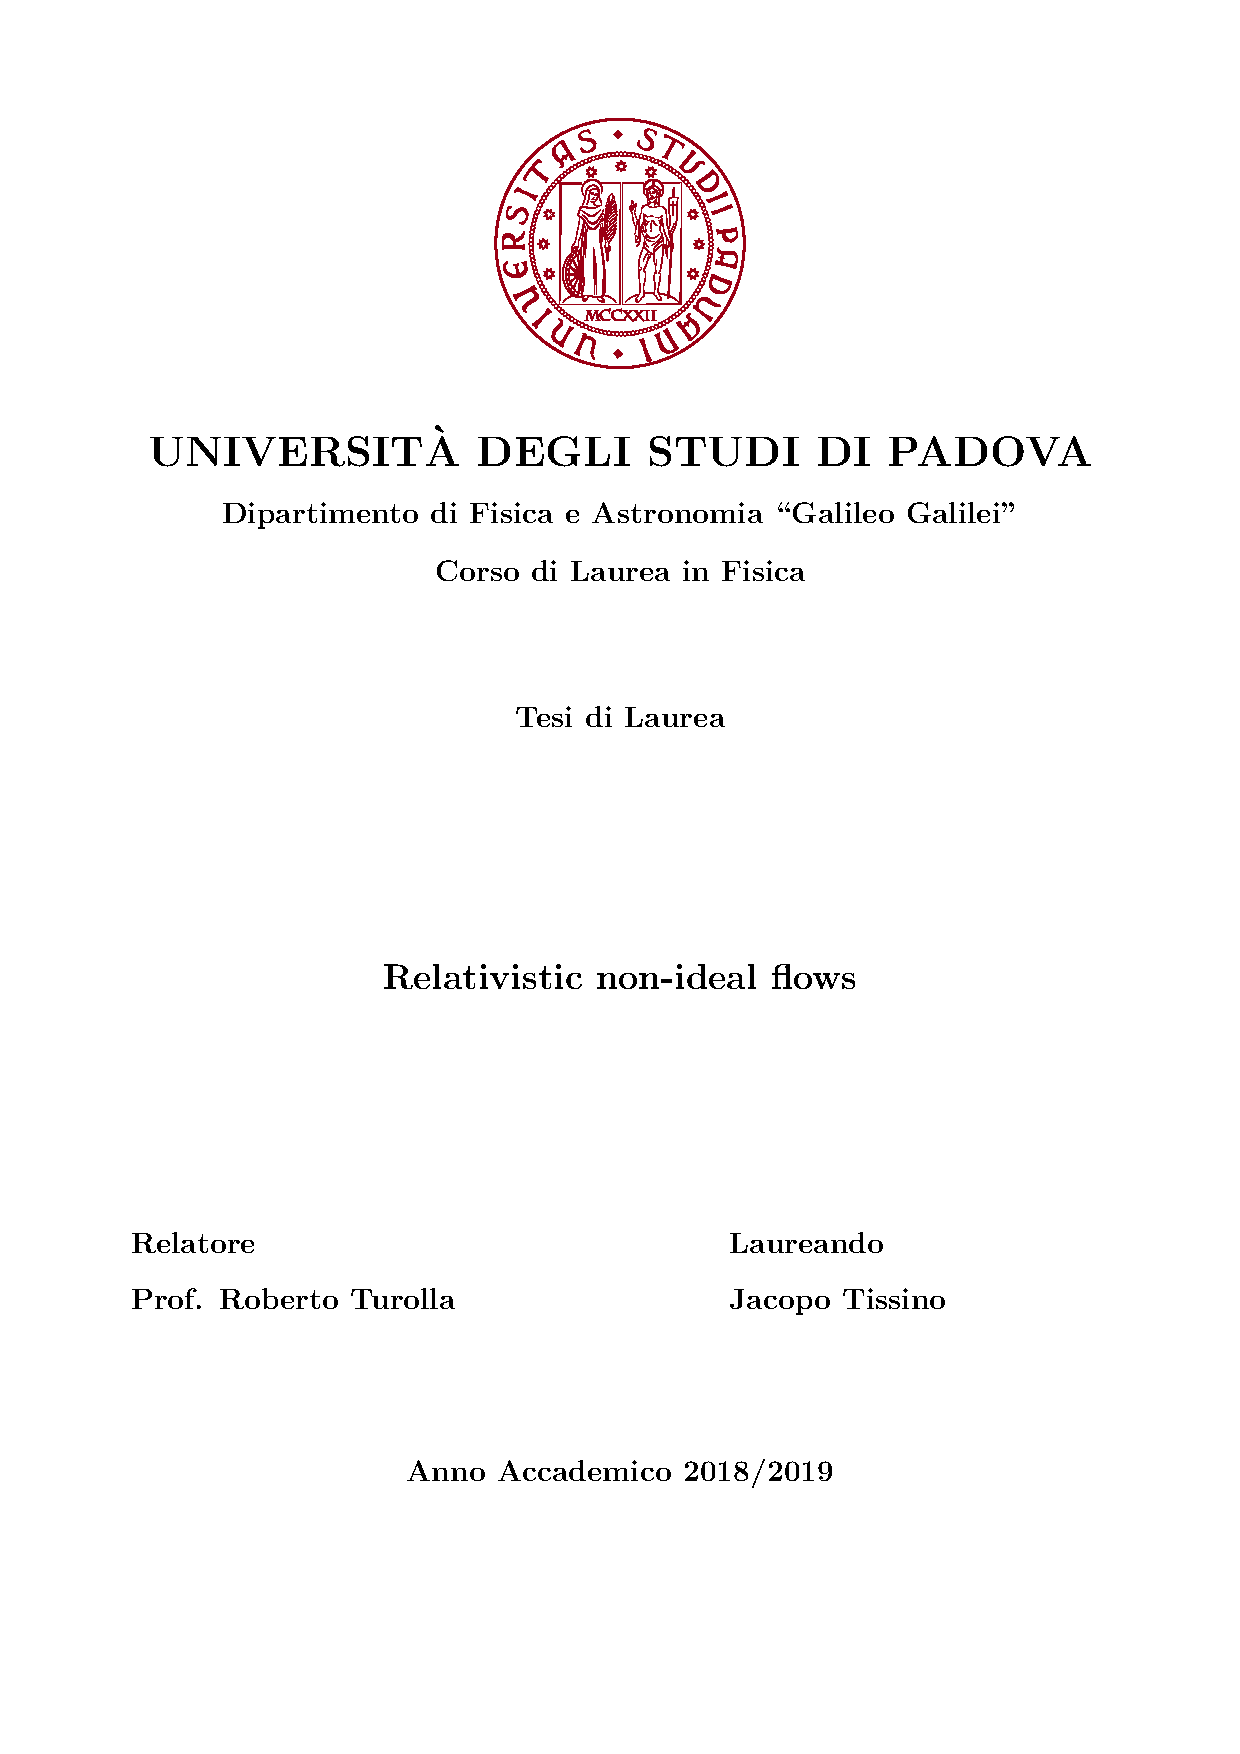
\includepdf[pages=1]{Frontespizio_Laurea.pdf}

\begin{abstract}
Stuff emits radiation when it falls into a black hole. I'd like to see exactly how much of it.
\end{abstract}

\section{Notational preface} \label{sec:notational-preface}

\subfile{conventions.tex}

\section{Useful formulas}

\subfile{formulas.tex}

\printbibliography[title={Bibliography}]

%\printindex

\end{document}
